% PARTIE 2 - TECHNIQUE %%%%%%%%%%%
% CHAPITRE 4 %%%%%%%%%%%%%%%%%%%%%
%%%%%%%%%%%%%%%%%%%%%%%%%%%%%%%%%%
Ce quatrième chapitre décrit le développement \textit{full-stack} de la carte, organisé en trois étapes. La première étape consiste à établir les fonctionnalités structurelles de la carte, incluant le fond de carte par défaut, le cartouche de la carte (titre, échelle, source, etc.), ainsi que les onglets destinés à accueillir les filtres, les images et la légende. Cet ensemble est réalisé à partir des fonctionnalités de la librairie Leaflet qu'il conviendra de définir. À ce stade, la carte n'est pas encore connectée à la base de données. La deuxième étape consiste à établir cette connexion via une \acrshort{api}, ce qui inclut la présentation de son fonctionnement et du requêtage asynchrone de l'application. L'\acrshort{api} permet ainsi de transmettre les données depuis la base jusqu'au \textit{front-end}. Une fois que les données sont prêtes pour être liées à la carte, elles doivent être réceptionnées et formatées pour être affichées et ordonnées afin de permettre à l'utilisateur une exploration interactive du projet Richelieu.  Il est important de noter que les propositions proposées dans ce chapitre sont provisoires, elles sont à l'état de brouillon. La carte présentée lors de la soutenance pourrait différer de celle présentée au cœur de ce chapitre, car le stage se termine après la date de soumission du mémoire.


%%%%%%%%%%%%%%%%%%%%%%%%%%%%%%%%%%%
% SECTION %%%%%%%%%%%%%%%%%%%%%%%%%
\section{Les fonctionnalités structurelles}
La carte est structurée en plusieurs éléments qui permettent son bon fonctionnement et son interaction avec l'utilisateur. Les modules qui la constituent sont développés avec la librairie Leaflet. 
% SUBSECTION %%%%%%%%%%%%%%%%%%%%%%%%%
\subsection{La librairie Leaflet}
\subsubsection{Définition et avantages}
Le projet Richelieu a fait le choix d'utiliser la librairie Leaflet pour réaliser la carte car elle présente plusieurs avantages. Il s'agit d'une bibliothèque JavaScript \textit{open source} conçue pour créer des cartes interactives. Les cartes créées en Leaflet sont compatibles avec les principaux navigateurs Web et adaptées aux environnements mobiles. La librairie est bien documentée par une communauté internationale\footnote{Le \href{https://leafletjs.com/plugins.html}{site} réunit une documentation très riche.} et active qui contribue à son amélioration. Leaflet est surtout connue pour sa prise en main facile pour tout développeur débutant : une simple carte Web peut être créée en quelques lignes de code. Parmi ses autres avantages, la librairie Leaflet est légère (le fichier JavaScript principal ne pèse que 42 kilooctets)\footnote{En informatique, la légèreté d'une librairie est importante car un fichier plus léger se charge plus rapidement dans le navigateur.} et performante (elle peut gérer des grandes quantités de données géospatiales sans surcharger les ressources du navigateur) car elle garantit des temps de chargement des données rapides. Sa flexibilité permet aussi l'intégration de nombreuses fonctionnalités grâce à des \textit{plugins} référencés sur le site de la librairie. Plusieurs zoom, des \textit{popups} ou encore les couches vectorielles sont possibles. Grâce à \acrshort{css}, ces éléments d'interface peuvent être facilement adaptés aux besoins graphiques de chaque projet. Ces avantages rendent Leaflet particulièrement adapté aux projets nécessitant des cartes interactives performantes et modulaires comme c'est le cas du projet Richelieu. 

\subsubsection{D'autres librairies et inconvénients}
Toutefois, il existe plusieurs librairies comparables à Leaflet pour la création de carte interactive sur le Web, mais elles présentent divers inconvénients. Par exemple, rares sont les librairies entièrement gratuites. L'\acrshort{api} JavaScript de Google Maps permet d'intégrer des cartes dans une application mais elle n'est pas \textit{open source}. MapBox GL JS offre une version gratuite, mais avec des fonctionnalités limitées. D'autres, comme OpenLayers et D3.js pour les plus connues, sont des librairies gratuites et complètes (riches en fonctionnalités et supportent de nombreux formats de données) mais elles nécessitent une longue courbe d'apprentissage. D3.js est par ailleurs plus orientée pour la visualisation de données au sens large que strictement pour la cartographie. Dans ce contexte, ces bibliothèques présentent des forces pour d'autres projets et des faiblesses pour le projet Richelieu.

Donc même si Leaflet présente plusieurs inconvénients car il n'est pas développé par un géographe et manque ainsi en rigueur, il reste le meilleur choix en raison de sa simplicité et de son adaptabilité pour développer les fonctionnalités qu'il convient à présent de présenter.  

% SUBSECTION %%%%%%%%%%%%%%%%%%%%%%%%%
\subsection{Les fonds de carte}
Toute carte géographique en ligne comporte au moins un fond de carte de référence, qui constitue une couche de base fournissant un contexte visuel et géographique. Ce fond de carte inclut des éléments d'arrière-plan tels que les routes, les limites administratives et les bâtiments. Il est placé en dessous des autres couches, qui viennent s'y superposer, et n'est généralement pas mentionné dans la légende. Les cartes sur le Web fonctionnent selon un système de superposition de couches, similaire aux cartes traditionnelles où l'on superpose un fond topographique avec des maillages administratifs, des frontières, des chemins de randonnée, des infrastructures ferroviaires et routières, ainsi que des espaces bâtis et naturels. Cette approche de modélisation géographique sur papier est transposée à la cartographie Web. 

\subsubsection{Des repères contemporains}
Leaflet propose un fond de carte par défaut mais il est possible de choisir celui qui correspond le mieux à nos besoins. Tandis que certains créent leur propre carte contemporaine, il existe un siteWeb qui recense de nombreux fonds existants (\href{https://leaflet-extras.github.io/leaflet-providers/preview/}{Leaflet Provider}). Certains fonds affichent les informations géographiques et topographiques, comme le détail du relief ou comme les bâtiments en \acrshort{3d} (voir~ le n°4 dans la figure \ref{fig:fond-carte-contemporain}), tandis que d'autres cartes adoptent un style inspiré de l'aquarelle (voir~ le n°5 dans la figure \ref{fig:fond-carte-contemporain}). Dans le cadre du projet Richelieu, nous avons restreint notre choix à quelques options adaptées un fond de carte urbain. Il est en effet essentiel que les rues et certains noms soient visibles, que les espaces verts soient discrètement représentés, et que l'information demeure lisible sans être trop claire ou trop sombre, tout en évitant des contrastes excessifs. 
\begin{figure}[h!]
    \centering
    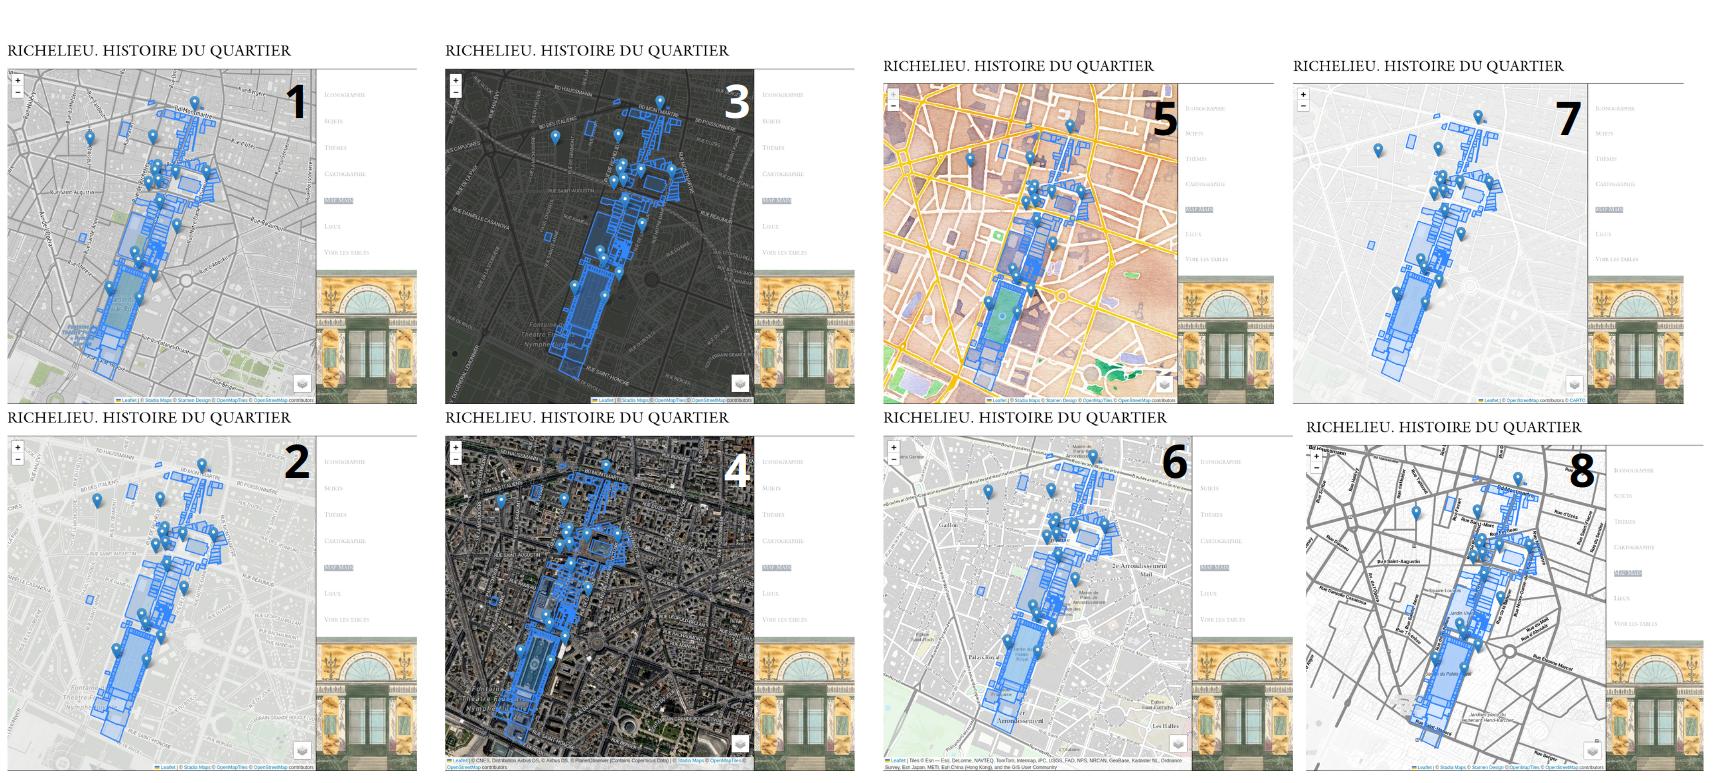
\includegraphics[width=1\linewidth]{images/fond-de-carte-contempo.png}
    \caption{Plusieurs propositions d'un fond de carte contemporain, \mhd.}
    \label{fig:fond-carte-contemporain}
\end{figure}
C'est pourquoi nous avons retenu le fond nommé World Topo Map, le n°6 de la figure \ref{fig:fond-carte-contemporain}. Il offre une bonne lisibilité des noms de rues, boulevards et squares, tout en restant clair. Ce fond de carte est équilibré, il n'y a pas de surcharge d'informations et l'espace n'en est pas trop dépouillé. Il a été conçu par la société internationale \acrshort{esri} (\textit{Environmental Systems Research Institute}), un acteur majeur dans le développement des  \acrshort{sig} appliqués à l'aménagement du territoire. Il est stocké par les serveurs de ArcGIS Online et se matérialise par une \acrshort{url}. Le fond de carte est donc une ressource du Web et externe à notre code mais qu'il convient d'inclure. 

Mais avant de se lancer dans les questions techniques d'ajout de fond de carte, une rapide présentation technique de Leaflet s'oblige. En Leaflet, une carte est stockée dans un objet \texttt{(L.map)} que l'on vient compléter, dans une approche modulaire, en y ajoutant d'autres objets Leaflet: des couches vectorielles, les popups, etc. Les données sont positionnées grâce à leur coordonnées géographiques. Il est ensuite possible de paramétrer des interactions avec la carte (click, scroll...) et donc de définir des scénarii de navigation. Enfin, Leaflet se charge de la production d'une visualisation cartographique en \acrshort{html}, à partir du code JavaScript utilisé pour produire la carte.

En Leaflet, un fond de carte est appelé \texttt{tileLayer} (souvent traduit de manière approximative par \enquote{couche de tuile}). On vient stocker l'\acrshort{url} dans une variable nommée \texttt{contemporain} ci-dessous que l'on ajoute à l'objet carte, \texttt{map}. De cette manière, le fond de carte est visible dès que la carte est chargée, c'est-à-dire dès que la page du navigateur Web est rafraîchie. Il convient de crééer l'objet \texttt{map} avant d'y ajouter une couche d'information.
 \begin{lstlisting}[language=PYTHON, caption=Variables et fonction d'initialisation de la carte en JavaScript]
 var map = L.map('map', {zoomControl:false}).setView([48.866772, 2.338935], 12);    
 
 var contemporain = L.tileLayer(
    'https://server.arcgisonline.com/ArcGIS/rest/services/World_Topo_Map/MapServer/tile/{z}/{y}/{x}', 
    {
        opacity: 1, 
        maxZoom: 18,
        minZoom: 12
    }
).addTo(map); 

 setTimeout(function(){
    map.flyTo([48.866772, 2.338935], 16);
 }, 4000);\end{lstlisting}
 
La création d'une \texttt{tileLayer} implique généralement de définir un niveau de zoom minimal et maximal, ainsi que des paramètres pour centrer la carte sur une localisation spécifique. 
Il est important de noter que Leaflet propose un grand nombre de paramètres, la plupart étant prédéfinis par défaut. Il revient donc au développeur de modifier ces paramètres par défaut afin que les interactions avec la carte correspondent aux spécifications souhaitées. Par exemple \texttt{zoomControl~:~false} désactive les contrôles de zoom par défaut (c'est-à-dire les boutons \enquote{~+~} et \enquote{~-~} que l'on peut généralement apercevoir sur une carte). A la place, il a été décidé de jouer pleinement avec les interactions offertes par Leaflet et JavaScript. 
Dans la première ligne de code, nous reconnaissons des coordonnées géographiques \texttt{48.866772, 2.338935} qui correspondent à un point géographique à Paris. Elles sont accompagnées d'un niveau de zoom \texttt{12} qui offre une vue intermédiaire permettant de visualiser toute la ville de Paris (voir~ \ref{fig:zoom-12}). A l'inverse, la fonction \texttt{setTimeout} augmente le niveau de zoom à \texttt{16} et offre une vue détaillée sur le quartier Richelieu (voir~ \ref{fig:zoom-16}). Cette transition est dynamique donnant un effet de \enquote{vol} vers la destination après 4 secondes d'attente au chargement de la carte.

\begin{figure}[h!]
    \begin{subfigure}{.5\textwidth}
      \centering
      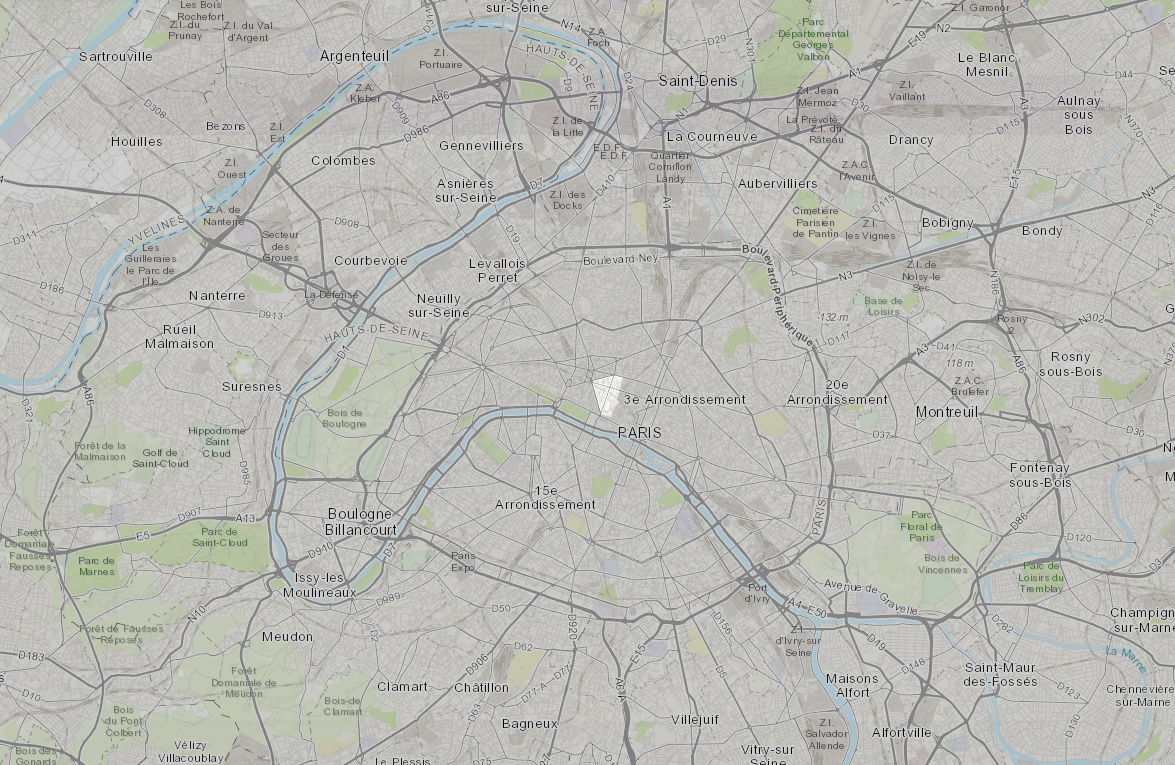
\includegraphics[width=0.7\linewidth]{images/zoom-12.png}
      \caption{Niveau de zoom à 12}
      \label{fig:zoom-12}
    \end{subfigure}
    \begin{subfigure}{.5\textwidth}
      \centering
      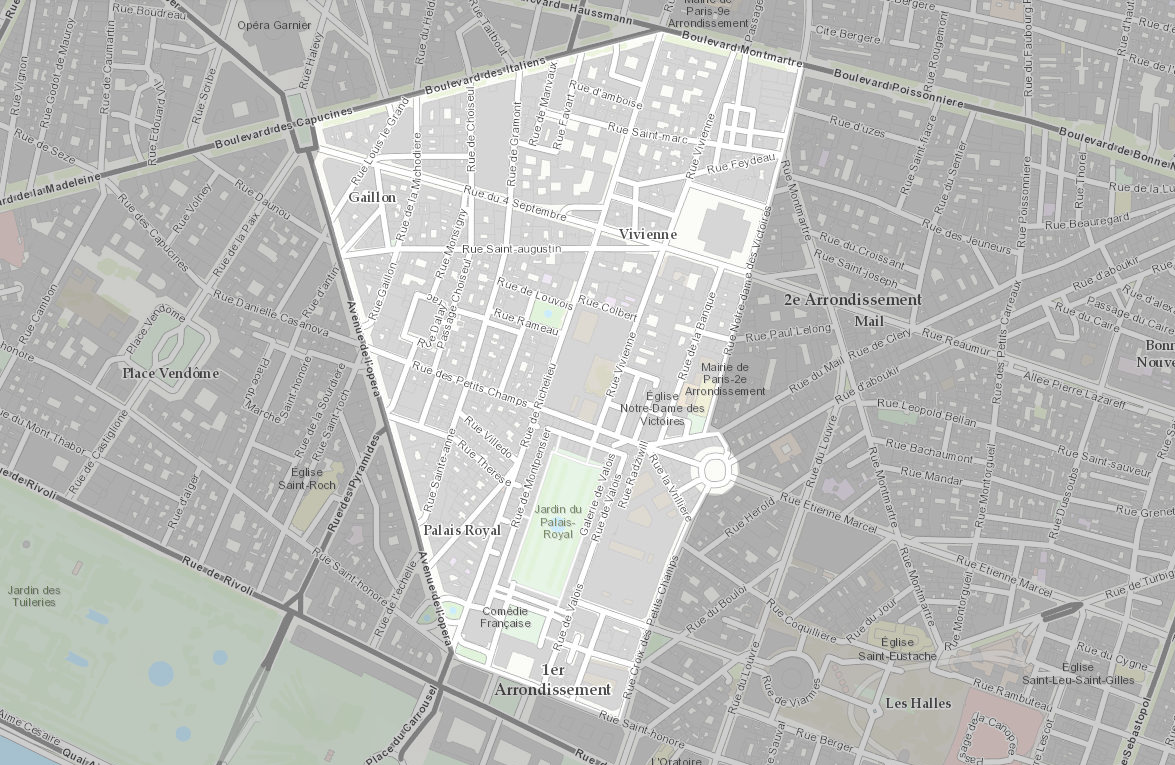
\includegraphics[width=.7\linewidth]{images/zoom-16.png}
      \caption{Niveau de zoom à 16}
      \label{fig:zoom-16}
    \end{subfigure}
\caption{Carte centrée sur Paris puis sur le quartier Richelieu}
\label{fig:zoom}
\end{figure}
Le zoom est un paramètre à ne pas négliger, car il peut influencer le choix du fond de carte. En effet, si le zoom n'est pas correctement limité et que l'utilisateur peut zoomer au maximum, le fond de carte risque de disparaître. Cela s'explique par le fait que les données ne sont pas disponibles à des niveaux de zoom très élevés, car les fonds de carte ont une résolution limitée. Il est donc nécessaire de restreindre les niveaux de zoom afin de gérer ces contraintes techniques.

Notons qu'un autre élément de repère est mis à disposition de l'utilisateur : en plus du zoom qui permet de situer le projet dans Paris, et plus précisément dans le quartier Richelieu, nous avons également délimité une zone spécifique pour le symboliser. Cette zone géographique vient personnaliser la carte en utilisant un objet \acrshort{geojson} qui applique un style spécifique. Il s'agit d'un \texttt{MultiPolygon}, soit une géométrie qui définit plusieurs polygones. Il y a donc un premier polygone qui vient recouvrir une partie de la carte (dont les limites paraissent invisibles car inaccessibles puisque le dézoom est restreint) et un second polygone qui correspond aux limites du quartier Richelieu comme définies par le projet. La première zone est remplie d'une couleur sombre pour donner un effet d'opacité. 

Ainsi, le fond de carte contemporain, le zoom interactif et les délimitations de l'emprise du quartier fournissent des repères spatiaux clairs. Ces premiers éléments ont été conçus pour aider l'utilisateur à interpréter plus facilement la carte et à accéder aux informations historiques tout en les contextualisant géographiquement. Par exemple, le zoom interactif montre que la carte n'est pas statique mais dynamique, incitant l'utilisateur à l'explorer, même avant que les données historiques ne soient affichées. De plus, nous pensons que l'inclusion de repères familiers, tels que les rues et les bâtiments actuels, permet d'établir un lien direct entre le présent et le passé. C'est pourquoi nous proposons d'ajouter un curseur d'opacité entre le fond de carte contemporain et les fonds de cartes historiques.

\subsubsection{Curseur d'opacité avec les fonds de cartes historiques}
Un curseur d'opacité permet de définir la transparence d'un élément, en l'occurrence le degré de visibilité d'un fond de carte.  Cette fonctionnalité ne s'applique pas au fond de carte contemporain, qui est la première couche de la carte, mais aux fonds de cartes historiques. Le curseur permet ainsi de passer du fond de carte contemporain au fond historique sélectionné, le premier servant ainsi de support à la spatialisation d'un phénomène. 
\begin{lstlisting}[language=PYTHON, caption=Variable qui stocke les fonds de cartes historiques en JavaScript]
 var tileLayers = {
      '1. Plan Verniquet (1791)': 'https://tile.ptm.huma-num.fr/tiles/ark/highres/12148/btv1b55013275x/{z}/{x}/{y}.Webp',
      '2. Atlas Vasserot (1810-1836)': 'https://tile.maps.huma-num.fr/uc2usU/d/Alpage_Vasserot_1830/{z}/{x}/{y}.png',
      '3. 1812': 'https://tile.ptm.huma-num.fr/tiles/ark/highres/12148/btv1b530851375/{z}/{x}/{y}.Webp',
      '4. Cadastre municipal (1900)': 'https://tile.maps.huma-num.fr/uc2usU/d/MOSA_1900_PARIS/{z}/{x}/{y}.png',
      '5. 1943': 'https://tile.ptm.huma-num.fr/tiles/ark/highres/12148/btv1b53121232b/{z}/{x}/{y}.Webp', 
    }\end{lstlisting}
    
Cette variable définit un objet JavaScript appelé \texttt{tileLayers} (le pluriel marque la distinction avec la couche initiale \texttt{tileLayer}), qui regroupe les couches de cartes historiques. Chaque entrée représente un fond de carte, identifié par son nom et sa date de création, associés à une \acrshort{url}. Ces \acrshort{url}s pointent vers des données hébergées sur les serveurs de Huma-Num. Certaines cartes ont été générées à l'aide des outils du \acrshort{cstptm}, notamment \acrshort{galligeo}, pour le géoréférencement des cartes de Gallica. Les cartes sélectionnées couvrent la période chronologique du projet. La plus ancienne date de 1791 (plan Verniquet) et la plus récente de 1943 (voir la figure \ref{fig:carto-histo}). Le principal défi dans le choix de ces cartes réside dans leur géoréférencement, qui doit correspondre le plus précisément possible aux données du \acrshort{sig}, sur lesquelles les polygones ont été dessinés. Toutefois, la numérisation des cartes historiques présente dans certains cas des décalages car le papier a été plié et le pli est numérisé, ainsi le polygone est \textit{de facto} décalé (comme en témoigne la figure \ref{fig:verniquet-décalage}). 
\begin{figure}[h!]
    \centering
    \includegraphics[width=0.2\linewidth]{images/décalage-bnf.png}
    \caption{Zoom plan Verniquet (1791), décalage géoréférencement}
    \label{fig:verniquet-décalage}
\end{figure}
Ces cartes sont ensuite ajoutées dans un contrôleur de couches \texttt{layersControl}, une fonctionnalité proposée par Leaflet. Par la suite, chaque carte est gérée via un \textit{slider} \acrshort{html} d'opacité qui permet de modifier directement la transparence de la couche active sélectionnée.
\begin{figure}[h!]
    \centering
    \includegraphics[width=0.5\linewidth]{images/opacité-vasserot-contempo-galerie-vivienne.png}
    \caption{Zoom galerie Vivienne avec faible niveau d'opacité de l'Atlas Vasserot}
    \label{fig:opacité-galerie}
\end{figure}
Cette fonctionnalité offre la possibilité de visualiser les transformations urbaines en superposant plusieurs cartes. Par exemple, la figure \ref{fig:opacité-galerie}  illustre cette utilisation : en haut à droite, le curseur d'opacité est réglé sur une faible valeur, laissant apparaître la carte Vasserot de manière partielle, ce qui permet de la comparer avec la carte contemporaine et de visualiser l'environnement bâti avant la construction de la galerie Vivienne. La figure \ref{fig:opacité-rueVivienne} montre quant à elle la superposition de cartes historiques, entre l'Atlas Vasserot et le cadastre municipal de 1900, pour laisser figurer dans le coin inférieur gauche le percement Nord de la rue Vivienne.
\begin{figure}[h!]
    \centering
    \includegraphics[width=0.5\linewidth]{images/opacité-vasserot-feuille-rue-vivienne.png}
    \caption{Zoom rue Vivienne avec faible niveau d'opacité du cadastre municipal}
    \label{fig:opacité-rueVivienne}
\end{figure} 

Ainsi structuré le code est actif, dynamique et réagit aux ajouts et suppressions de couches que sélectionne l'utilisateur. L'opacité et la visibilité des couches sont ajustées en temps réel sur la carte. Surtout, des informations historiques sont déjà figurées alors qu'aucune connexion à la base de données n'ait  encore effectuée.

% SUBSECTION %%%%%%%%%%%%%%%%%%%%%%%%%
\subsection{Le cartouche : les éléments constitutifs de la carte}
La carte est habillée d'éléments constitutifs, obligatoires dans la cartographie classique, vivement recommandés pour la cartographie Web. Ces éléments sont le titre, la source, la date de création, l'échelle et la légende. D'autres éléments sont facultatifs tels que l'orientation, le cartouche autour de la carte, les toponymes, le quadrillage des coordonnées géographiques (graticule). 
\subsubsection{Le titre, la source et la date}
Le titre, la source et la date sont des éléments qui sont définis par défaut par Leaflet. Il est toutefois possible de modifier les crédits, d'ajouter un hyperlien vers le projet. Les éléments suivants sont facilement modifiables :
\begin{lstlisting}[language=PYTHON, caption=Changement des attributions de la carte en JavaScript]
map.attributionControl.setPrefix('<a href="https://leafletjs.com/">Leaflet</a>');
map.attributionControl.addAttribution('&copy; <a href="https://quartier-richelieu.inha.fr/">Richelieu.Histoire du quartier</a>, Marina Hervieu, 2024');\end{lstlisting}

\subsubsection{L'échelle et l'orientation}
L'échelle et l'orientation sont des éléments issus de plugins. Avec Leaflet, un plugin est une extension qui ajoute des fonctionnalités supplémentaires à la bibliothèque de base. Ils peuvent être développés par la communauté ou par les créateurs de Leaflet, et sont utilisés pour enrichir les cartes interactives avec des options qui ne sont pas incluses dans le cœur de la bibliothèque. Un plugin s’ajoute généralement en important un fichier JavaScript et une feuille de style \acrshort{css} (s'ils sont fournis) dans le projet, puis en initialisant ses fonctionnalités dans le code. 
Voici les plugins (seul le code JavaScript est ajouté) pour l'échelle (\texttt{scale}) et l'orientation (\texttt{compas}):
\begin{lstlisting}[language=PYTHON, caption=Plugins échelle et orientation en JavaScript]
L.control.scale({position:'bottomleft'}).addTo(map);
var compass = L.control.compass({
    position: 'topright',
    autoActive: true  
}).addTo(map); \end{lstlisting}
En complément des lignes de code JavaScript, des modifications sont à apporter dans le code \acrshort{html}, il s'agit de références aux fichiers \acrshort{css} dans le \texttt{<head>} et dans le \texttt{<script>} de JavaScript. Il est à noter que ces fonctionnalités ne sont pas toujours intuitives et que leur implémentation peut entraîner des problèmes de compatibilité. Par exemple, l'orientation a été développée en 2014 avec une version antérieure de Leaflet que celle utilisée acutellement, rendant le plugin initial obsolète. La mise à jour des plugins par la communauté permet cependant de les réutiliser. C'est probablement pour cette raison technique que la plupart des cartes sur le Web ne les intègrent pas, car cela implique de consulter davantage la documentation de Leaflet pour les implémenter correctement.

\subsubsection{Les onglets : la légende et le point \enquote{à propos}}
Enfin, pour faciliter l'ajout d'information sans affaiblir la visibilité de la carte, des onglets comportant la légende et un \enquote{à propos} ont été développés. Il s'agit de panneaux latéraux communément appelés \texttt{sidebar}. 
Au chargement de la carte, un onglet \enquote{à propos} apparaît afin d'expliquer dans les grandes lignes l'objet de la carte et son utilisation. Il se ferme et reste à disposition en haut à gauche, sous le titre de la carte. 
\begin{figure}[h!]
    \centering
    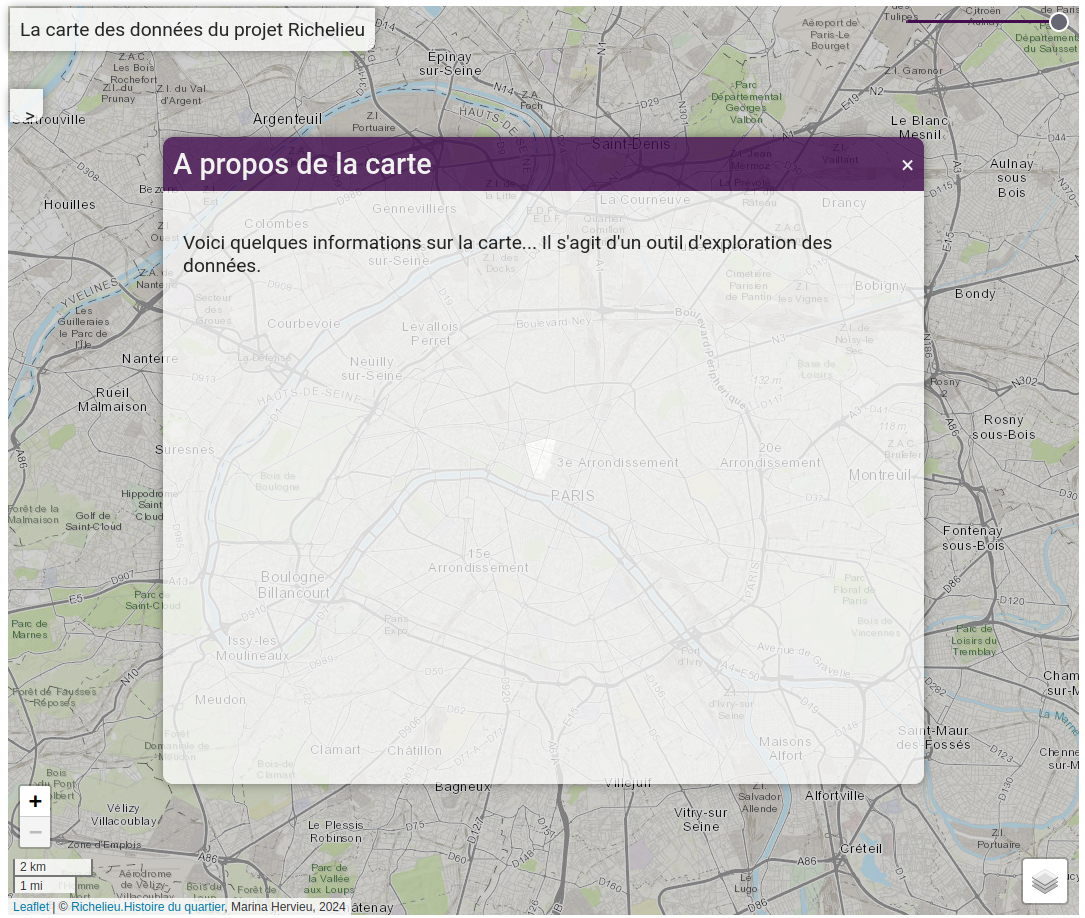
\includegraphics[width=0.75\linewidth]{images/a-propos.png}
    \caption{Onglet \enquote{à propos} au chargement de la carte}
    \label{fig:a-propos}
\end{figure}

L'onglet \enquote{Légende} se trouve quant à lui juste en dessous et enregistre les premiers éléments de légende codés, tels que les couleurs des polygones. Ces onglets sont à considérer comme de nouvelles pages \acrshort{html} que l'on vient ajouter à la carte, la couche initiale. C'est seulement après coup, que nous avons constaté qu'il existe un plugin \texttt{sidebar} développé par Leaflet. A terme, il serait souhaitable de réécrire le code écrit \textit{from scratch} pour l'intégrer via ce plugin certainement plus efficace. 

Pour conclure, les repères contemporains et les éléments structurels sur une carte historique facilitent la compréhension, l'accessibilité, et l'engagement des utilisateurs en leur offrant un cadre spatial connu\footnote{On estime que les utilisateurs de la carte auront \textit{a minima} connaissance de la situation de Paris en tant que capitale de la France} tout en permettant une exploration des données historiques dans un contexte innovant et interactif. Tout l'enjeu de la cartographie Web réside dans ces \enquote{deux fonctions importantes d’une carte : \enquote{susciter des émotions} et \enquote{ancrer dans la réalité}. C’est donc à l’égard de ces deux fonctions que les mondes virtuels peuvent enrichir les représentations cartographiques symboliques. En suscitant des émotions, ils captivent l’attention du lecteur. En ancrant la représentation dans la réalité, ils favorisent la prise de conscience.}\footcite{BUCHERcarte2007}
%%%%%%%%%%%%%%%%%%%%%%%%%%%%%%%%%%%
% SECTION %%%%%%%%%%%%%%%%%%%%%%%%%
\section{Du \textit{back-end} au \textit{front-end}: les requêtes avec l'\acrshort{api}}
Cette section détaille précisément le processus par lequel les données stockées dans la base de données sont requêtées, récupérées et ensuite affichées sur la carte grâce à l'\acrshort{api}, dont le fonctionnement sera présenté. Ce processus est notamment indispensable pour connecter les données à la carte réalisée et présentée dans la précédente section. 
% SUBSECTION %%%%%%%%%%%%%%%%%%%%%%%%%
\subsection{Le fonctionnement d'une \acrshort{api} REST}
\subsubsection{Définition et principes}
Une \acrshort{api}, \textit{Application programming interface} ou interface de programmation d'application permet la communication entre des ressources via une architecture Web de type client-serveur, structurée pour organiser les services en ligne. L'\acrshort{api} repose sur le protocole \acrshort{http} (\textit{HyperText Transfer Protocol}), dont le rôle est de définir les règles de communication entre le client et le serveur\footcite{KERVEGANModelisation2022}. La principale différence entre \acrshort{http} et une \acrshort{api} est que le premier est un protocole générique pour le Web, tandis que l'\acrshort{api} est spécifique à un projet, comme une application, un logiciel ou un ensemble d'applications. Il existe des standards d'interaction entre client et serveur, comme l'\acrshort{api} REST, développée en 2000 par Roy Fielding\footcite{FIELDINFarchitectural2000}. Ce standard est étroitement lié au protocole \acrshort{http}, conçu par le même ingénieur. En somme, l'\acrshort{api} est un code, une "langue" permettant aux machines de communiquer, et elle peut être développée dans des langages tels que Python ou JavaScript.

L'\acrshort{api} REST repose sur plusieurs principes fondamentaux que le projet Richelieu a mis en œuvre. Dans le cadre de cette application, qui utilise PostgreSQL pour le stockage des données, Flask pour la gestion de la logique serveur, et Leaflet pour l'affichage de données cartographiques, l'\acrshort{api} REST organise les interactions entre ces différents composants. Flask expose des routes qui servent de points d'accès aux ressources, permettant d'accéder aux données géospatiales stockées dans PostgreSQL. Chaque route, accessible par des méthodes \acrshort{http} telles que \acrshort{get} ou \acrshort{post}, permet au client (la page \acrshort{html} avec Leaflet) d'effectuer des opérations sur ces données, comme la récupération ou la modification de polygones représentant des zones géographiques, tout en respectant les principes REST. Ces principes incluent une \acrshort{api} sans état  (\textit{stateless}), l'utilisation de méthodes \acrshort{http} standards (\acrshort{get}, \acrshort{post}, PUT, \acrshort{delete}), et l'interaction avec des ressources identifiables via des\acrshort{uri} (\textit{Uniform Resource Identifier}). Chaque requête contient ainsi toutes les informations nécessaires pour être traitée par le serveur, sans maintenir d'état entre les requêtes. Les réponses sont généralement fournies en format \acrshort{json}ou GeoJSON. Plus largement, l'\acrshort{api} REST est devenue très populaire depuis le début des années 2000 (notamment chez Salesforce, Amazon, Google), car elle consomme moins de bande passante, ce qui en fait une solution plus efficace pour les applications en ligne.

\subsubsection{Le requêtage asynchrone}
Le requêtage asynchrone dans ce contexte permet à l'application Web d'envoyer des requêtes à l'\acrshort{api} REST de Flask pour interagir avec les données stockées dans PostgreSQL sans interrompre le fonctionnement de l'interface utilisateur. La requête asynchrone est étroitement liée à l'\acrshort{api} REST dans le sens où elle permet de faire des appels \acrshort{http} à l'\acrshort{api} sans bloquer le fil d'exécution principal de l'application cliente. Une requête asynchrone via JavaScript (par exemple avec \texttt{Fetch API}) permet au client d'envoyer une requête à l'\acrshort{api} REST et d’attendre la réponse tout en continuant à fonctionner. Cela améliore considérablement la réactivité de l'interface utilisateur. Pendant que les données sont récupérées, l'utilisateur peut continuer à interagir avec la page, sans attendre un rechargement complet de celle-ci. Ces deux concepts  interagissent étroitement dans l'application : 
\begin{itemize}
    \item \acrshort{api} REST : La page Leaflet envoie une requête \acrshort{http} (via \acrshort{get} par exemple) à l'\acrshort{api} REST fournie par l'application Flask pour obtenir des données (comme des polygones représentant des lieux).
    \item Requête asynchrone : Cette requête est envoyée de manière asynchrone grâce à Fetch \acrshort{api} en JavaScript, ce qui permet à la page de continuer à fonctionner pendant que les données sont récupérées. 
    \item Réponse \acrshort{json}(ou GeoJSON) : Une fois que Flask a traité la requête et récupéré les données depuis PostgreSQL (en utilisant SQAlchemy dans notre cas), il renvoie les données de nouveau au format \acrshort{json}(ou GeoJSON) à la page \acrshort{html}. 
    \item Affichage des données : Leaflet prend le relais pour afficher les données sur la carte, et tout cela sans aucune interruption visible ou délais de traitement des données pour l'utilisateur de la carte. 
\end{itemize}
Donc l'\acrshort{api} REST fournit des points d'accès (\textit{endpoints}) qui permettent d'interagir avec les ressources (données) sur le serveur, tandis que la requête asynchrone permet d'interagir avec ces points d'accès de façon \enquote{décalée} pour améliorer la fluidité et réactivité de l'application Web. 

% SUBSECTION %%%%%%%%%%%%%%%%%%%%%%%%%
\subsection{Une route de l'application en guise d'exemple}\label{sous-section:fetch-api-places}
Cette route Flask ci-dessous (voir Listing 4.5) expose une \acrshort{api} REST et démontre une requête asynchrone pour récupérer et retourner les données iconographiques d'un lieu en GeoJSON. Détaillons le code pour approfondir la compréhension des principes. 
\begin{lstlisting}[language=PYTHON, caption=Route get-places pour chercher les données iconographiques liées aux lieux et préparer le format de données à envoyer au front-end]
@app.route('/api/places', methods=['GET'])
def get_places():
    # Récupérer tous les lieux
    places = Place.query.all()

    #Variable pour stocker les GeoJSON des lieux
    places_geojson = []

    # Boucle sur chaque lieu
    for place in places:
        # Requête distincte pour récupérer les iconographies associées à ce lieu
        r_iconography_places = R_IconographyPlace.query.filter_by(id_place=place.id).all()
        iconographies = [r.iconography for r in r_iconography_places]
        iconography_count = len(iconographies)  # Compter le nombre d'iconographies pour chaque lieu

        # Utiliser fonction serialize_full 
        iconography_data = [iconography.serialize_full() for iconography in iconographies]

        # Créer la structure GeoJSON pour chaque lieu
        place_data = {
            "type": "Feature",
            "properties": {
                "id": place.id,
                "name": place.id_richelieu,
                "iconography_count": iconography_count,
                "iconographies": iconography_data
            },
            "geometry": place.vector  # La géométrie du lieu en GeoJSON
        }
        places_geojson.append(place_data)

    # Retourner une FeatureCollection sous format GeoJSON
    return jsonify({
        "type": "FeatureCollection",
        "features": places_geojson
    })\end{lstlisting}
L'\acrshort{api} REST est exposée via la route \texttt{@app.route('/api/places', methods=['GET'])} dont \texttt{'/api/places'} est le point d'accès. Elle permet à l'application cliente d'envoyer des requêtes \acrshort{http} \acrshort{get} à l'\acrshort{api} pour récupérer les informations sur les lieux et leurs iconographies associées. Les données sont clairement exposées sous forme de ressources, et chaque lieu est une ressource représentée par un GeoJSON que le client demande. En effet, celui-ci envoie une requête asynchrone via la fonction JavaScript \texttt{fetch()} pour récupérer les données. Les données stockées sont traitées via une requête \acrshort{sql} et un formatage. Le serveur Flask interroge la base de données PostgreSQL via SQLAlchemy pour récupérer les lieux (\texttt{Place.query.all()}) et, pour chaque lieu, il récupère les iconographies associées via la table de relation \texttt{R\_IconographyPlace}. Pour chaque lieu, les données sont organisées dans une structure GeoJSON, qui comprend les informations géométriques (via \texttt{place.vector}) ainsi que les propriétés du lieu, comme son ID, son nom, et les iconographies associées via \texttt{serialize\_full} (une fonction prédéfinie pour récupérer toutes les informations telles que les métadonnées des iconographies) ainsi qu'un compte du nombre d'iconographies par lieu. L'ensemble de ces informations sont ensuite retournées par le serveur dans une \texttt{FeatureCollection} GeoJSON, un format adapté à des bibliothèques comme Leaflet pour afficher des données géospatiales sur une carte. La réponse est encapsulée dans un format \acrshort{json}via \texttt{jsonify()}, respectant les standards de l'\acrshort{api} REST. 

Cette route est un exemple parmi d'autres codes développés pour interagir avec les données à préparer pour la carte. La prochaine étape du développement de l'outil consiste à tester la requête pour s'assurer que les données GeoJSON sont correctement récupérées d'une part, et correctement affichées sur la carte d'autre part. 
%%%%%%%%%%%%%%%%%%%%%%%%%%%%%%%%%%%
% SECTION %%%%%%%%%%%%%%%%%%%%%%%%%
\section{L'affichage des données}
L'affichage des données relève du \textit{front-end} de l'application. Cette section présentera quelques exemples de visualisation des données ainsi quelques éléments du code développé pour les réaliser. 
% SUBSECTION %%%%%%%%%%%%%%%%%%%%%%%%%
\subsection{Le lieu figuré par les parcelles}
Le lieu, en tant qu'entité principale du modèle de données du projet Richelieu, est représenté par un ensemble de géométries définies par des coordonnées géographiques. Ces géométries peuvent prendre la forme de polygones, qui représentent une surface fermée définie par plusieurs paires de coordonnées, la première et la dernière devant être identiques pour former un polygone fermé. Dans d'autres cas, lorsque les lieux représentent une rue ou un point d'intérêt, ils sont définis par un point unique avec une seule paire de coordonnées. Ensemble, ces éléments constituent les parcelles à positionner sur la carte, à partir desquelles l'exploration des données s'effectue.

\subsubsection{De l'affichage par défaut à la personnalisation}
Leaflet utilise de nombreux paramètres par défaut pour afficher les données, notamment dans le cas des lieux. Cependant, il est nécessaire de spécifier dans le formatage des données le type de géométrie : les polygones sont des \texttt{vector}, tandis que les points sont des \texttt{centroid}, sachant que chaque polygone possède également un point central, calculé automatiquement par défaut - ci-dessous un extrait de données au format GeoJSON.  

\begin{lstlisting}[language=PYTHON, caption=Structure GeoJSON]
{
   "type": "FeatureCollection",
   "features": [
       {
          "type": "Feature",
          "geometry": {
            "type": "Point",
            "coordinates": [  
                2.339712423376673,
                48.86822533019579
                ],
          },
          "properties": {
            "title": "Rue Vivienne"
          }
        },
        {
          "type": "Feature",
          "geometry": {
            "type": "Polygon",
            "coordinates": [
              [
                [
                  2.337516076011978,
                  48.86677742624936
                ],
                [
                  2.3382407144394213,
                  48.868162909802265
                ],
                [
                  ...
                ],
                [
                  2.337516076011978,
                  48.86677742624936
                ]
              ]
            ],
          },
          "properties": {
            "title": "2 Rue Vivienne"
          }
        }
    ]
}
\end{lstlisting}
À partir de ce fichier reçu par le client, celui-ci propose un affichage par défaut: il expose la donnée via des points (voir la figure \ref{fig:2eme-affichage}) plutôt que par des polygones, il convient de lui préciser le formatage des données attendu afin de l'afficher comme illustré (voir figure \ref{fig:1er-affichage}), par exemple. 

\begin{figure}[h!]
    \begin{subfigure}{.5\textwidth}
      \centering
    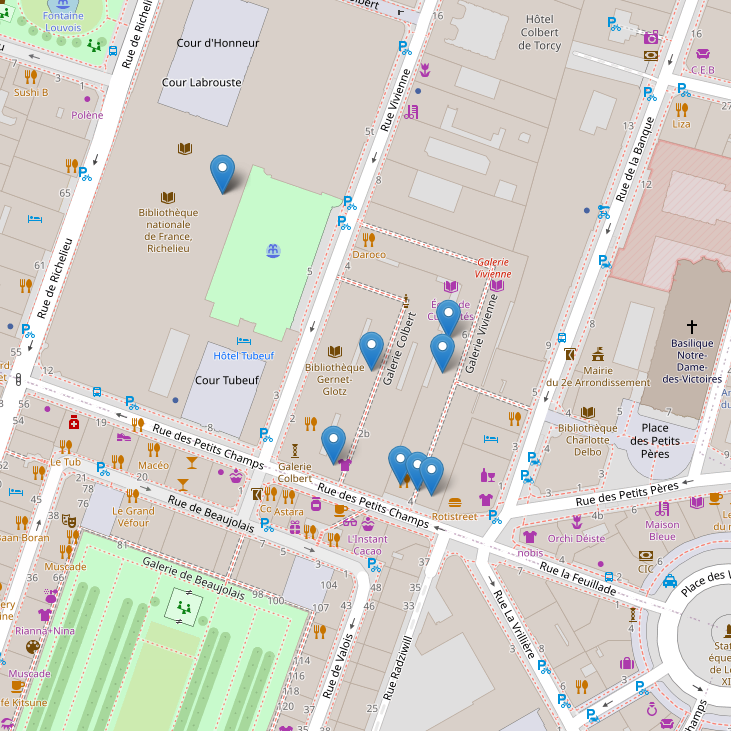
\includegraphics[width=.7\linewidth]{images/1er-affichage.png}
    \caption{Sans formatage précisé}
    \label{fig:2eme-affichage}
    \end{subfigure}
    \begin{subfigure}{.5\textwidth}
      \centering
      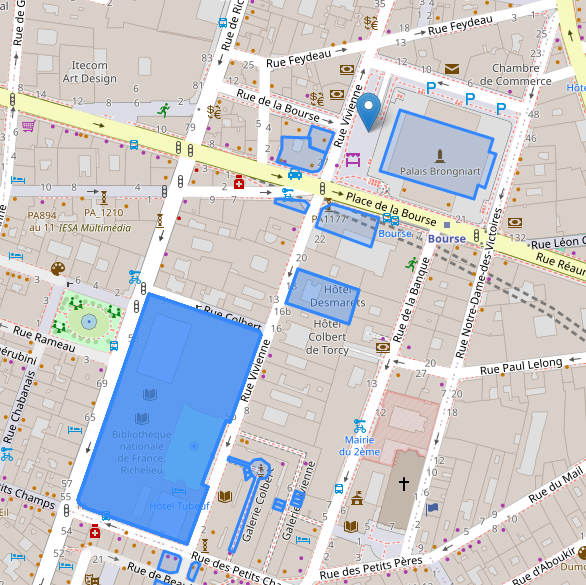
\includegraphics[width=0.7\linewidth]{images/2eme-affichage.png}
    \caption{Avec formatage précisé}
    \label{fig:1er-affichage}
    \end{subfigure}
    \caption{Exemple d'affichage sans et avec formatage précisé des données de lieux}
\label{fig:affichage-defauts}
\end{figure}

\subsubsection{La fonction \texttt{fetch}}
Pour ce faire, on utilise la fonction \texttt{fetch} en JavaScript car elle permet d'effectuer des requêtes \acrshort{http} asynchrones vers un serveur, pour récupérer des données, généralement au format JSON, ou envoyer des données. Elle est très souvent utilisée pour obtenir et traiter des informations sans avoir à recharger la page, comme dans l'exemple où le client, l'application, doit récupérer des polygones ou des points. \texttt{fetch} prend comme premier paramètre l'\acrshort{url} de la ressource à récupérer, et retourne la réponse. Une fois la réponse reçue, il est possible de l'exploiter, par exemple en la convertissant en GeoJSON pour un traitement ultérieur. 
\begin{lstlisting}[language=HTML, caption=Exemple d'utilisation de la fonction fetch]
fetch('/api/places')
  .then(response => response.json()) 
  .then(data => {
    L.geoJSON(data).addTo(map); 
  })
  .catch(error => console.error('Erreur lors de la récupération des données:', error));
\end{lstlisting}

La requête \texttt{fetch('/api/places')} envoie une requête \acrshort{get} à l'\acrshort{api} REST, elle demande à avoir les données sur les lieux exposées par Flask. La réponse est ici convertie en \acrshort{json}avec \texttt{response.json()} et les données récupérées sont ajoutées à la carte Leaflet via la ligne \texttt{L.geoJSON(data).addTo(map);}. Au même titre que la fonction \texttt{print()} en Python, le \texttt{console.log} est une technique constamment utilisée pour afficher des informations, un message ou des repères sur la console du navigateur Web (accessible par \texttt{ctrl + i}).

\subsubsection{Le type de données}
Il est cependant important de bien interpréter la nature des données récupérées, car celles-ci correspondent à des représentations géographiques spécifiques. Dans la mesure où la donnée du lieu est représentée par des parcelles géographiques, il convient de préciser qu'elles correspondent à un type particulier de donnée. Les polygones sont des données qualitatives nominales zonales, c'est-à-dire des surfaces délimitées, comme nous l'avons défini au cours du chapitre précédent avec le choix porté sur une carte choroplèthe (voir chapitre \ref{section:choix-carto}). En revanche, lorsque les lieux sont représentés par des points, ils relèvent de données qualitatives ponctuelles. Les données qualitatives nominales sont un type de données qualitatives (ou catégoriques) qui servent à classer ou identifier des éléments en fonction de catégories ou de labels, sans ordre particulier. Elles sont non numériques et ne possèdent aucune hiérarchie ou relation d'ordre entre les catégories. Chaque catégorie est unique même si les lieux peuvent être classés par type (parcelle, aile, ensemble, rue, etc.). L'objectif est simplement de distinguer les différents éléments ou groupes, sans qu'il y ait une notion de quantité ou d'intensité. Par exemple, les couleurs (rouge, vert, bleu) sont différentes et ne représentent aucun ordre. Ainsi les polygones n'ont pas de relation d'ordre entre eux, mais il est toutefois possible de classer visuellement les zones sur la carte, nous verrons en détail ce point par la suite. Surtout, ces distinctions sont essentielles pour interpréter correctement la nature des données géographiques et leur représentation visuelle sur la carte. 

% SUBSECTION %%%%%%%%%%%%%%%%%%%%%%%%%
\subsection{Mettre en scène les données}
Une fois que la communication des données entre le \textit{front-end} et le \textit{back-end } est mise en place dans l'application et assimilée par le développeur, il convient de les mettre en scène en exploitant autant que possible les langages du Web (\acrshort{html}, \acrshort{css} et JavaScript).
\subsubsection{Une question de d'échelle : les niveaux de granularité}
Nous avons vu lors du chapitre sur la modélisation de la donnée (voir \ref{sous-section:modele-bddr}) que les sources cartographiques sont réparties par niveaux de granularité. Nous avons ainsi tenté de proposer une première exploration des données à travers ce paramètre.
\begin{lstlisting}[language=PYTHON, caption=Récupérer les données cartographiques par granularité]
@app.route('/i/fetch-carto/', methods=['GET'])
def fetch_carto():
    '''
    fetch données cartographiques et retourner dans un GeoJSON Feature Collection 
    '''
    #méthode .split() utilisée pour séparer les arguments requêtés par le front
    
    carto = request.args.get('carto', '').split(' ')
    granularity = request.args.get('granularity', '').split(' ')
    print('%%', carto, granularity)
    r = db.session.execute(text("SELECT * FROM cartography;"))
    print(r.all())

 
    def feature_factory(cartography) -> dict:
        '''
        obtenir un objet cartographique et le retourner 
        '''
        return { "type":"Feature",
                 "geometry":cartography.vector,
                 "properties": { "id_uuid": cartography.id_uuid,
                                  "map_source": cartography.map_source,
                                  "granularity" : cartography.granularity                                  
                                  } } 
                                  
    #requête avec liste compréhensive
    #* décompose la liste compréhension en arguments
    #and_ garantit que les deux conditions sont vraies pour cartography.granularity&cartography.map_source
    #pour chaque combinaison, générer une condition de filtrage
    r = db.session.query(Cartography).filter(
        or_(*[
            and_(Cartography.granularity == grain, Cartography.map_source == cart)
                for grain in granularity  
                for cart in carto  
            ])
        )
    features = [ feature_factory(cartography) for cartography in r.all() ]
    print('%%%%%%%%%%', r)
    feature_collection = { "type": "FeatureCollection", "features": features }

    return jsonify(feature_collection)
\end{lstlisting}

\sloppy La fonction \texttt{fetch\_carto()} est accessible via l'\acrshort{url} \texttt{/i/fetch-carto/} qui utilise la méthode \acrshort{http} \acrshort{get}. Elle récupère des objets cartographiques filtrés par \texttt{carto} et \texttt{granularity} depuis la base de données. Les arguments passés dans l'\acrshort{url} (par exemple, \texttt{/i/fetch-carto/?carto=example\&granularity=detail)} sont récupérés par \texttt{request.args.get()}. Les arguments \texttt{carto} et \texttt{granularity} sont séparés en listes à l'aide de la méthode \texttt{.split(' ')}. Cela permet de traiter plusieurs valeurs passées dans l'\acrshort{url} en une seule chaîne de caractères, séparées par des espaces : \texttt{carto = ['exemple1', 'exemple2']} et \texttt{granularity = ['ensemble', 'aile']}. Puis la fonction \texttt{feature\_factory()} prend en argument un objet cartographique et le formate en GeoJSON. Elle renvoie ainsi le dictionnaire (\enquote{clé:valeur}) contenant le type de géométrie de l'objet, la géométrie en question et ses propriétés comme la granularité. 

Ensuite, une requête avec SQLAlchemy filtre les données en fonction des arguments passés dans l'\acrshort{url}. La condition \texttt{or\_(*[...])} recherche toutes les combinaisons possibles entre \texttt{carto} et \texttt{granularity} - un premier développement a essayé de résoudre ce point manuellement mais il s'est avéré incomplet. Cette condition assure que les deux conditions (granularity et map\_source) soient remplies pour chaque combinaison. La boucle imbriquée permet de générer les combinaisons et d'appliquer ces conditions de filtrage.

Nous estimons que ce paramètre permet de comprendre les différentes échelles de représentation figurées dans les sources qui reflètent la réalité bâtie. Une première visualisation offre à l'utilisateur la possibilité de sélectionner la granularité souhaitée, comme en témoigne les figures \ref{fig:gran-parcelle} et \ref{fig:gran-galerie}.  Il convient de noter que cet exemple repose sur une version préliminaire de la base de données, qui ne reflète pas encore le corpus final des données ; par exemple, la Banque de France n'y est pas encore incluse. 
\begin{figure}[h!]
    \begin{subfigure}{.5\textwidth}
      \centering
    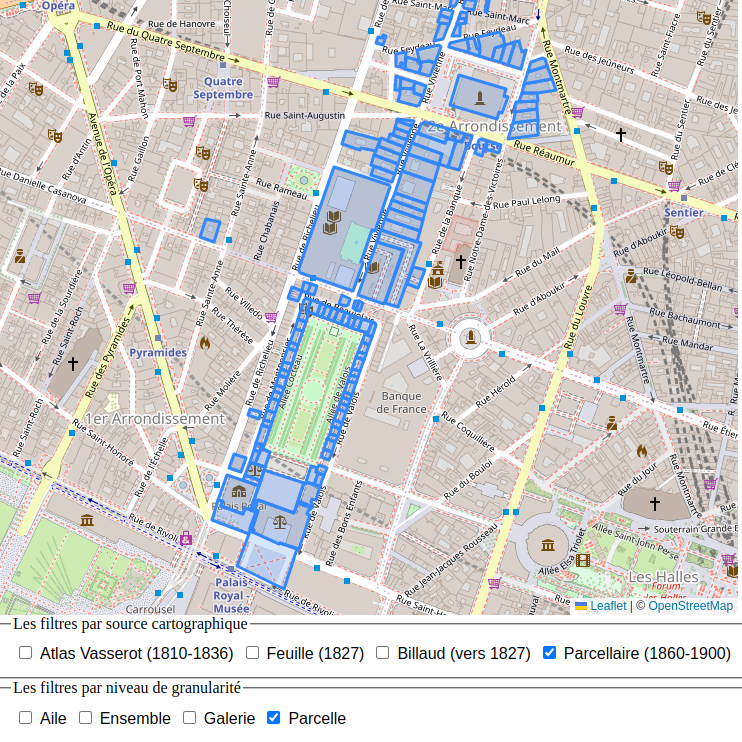
\includegraphics[width=.7\linewidth]{images/gran-parcelle.png}
    \caption{Affichage par parcelle}
    \label{fig:gran-parcelle}
    \end{subfigure}
    \begin{subfigure}{.5\textwidth}
      \centering
      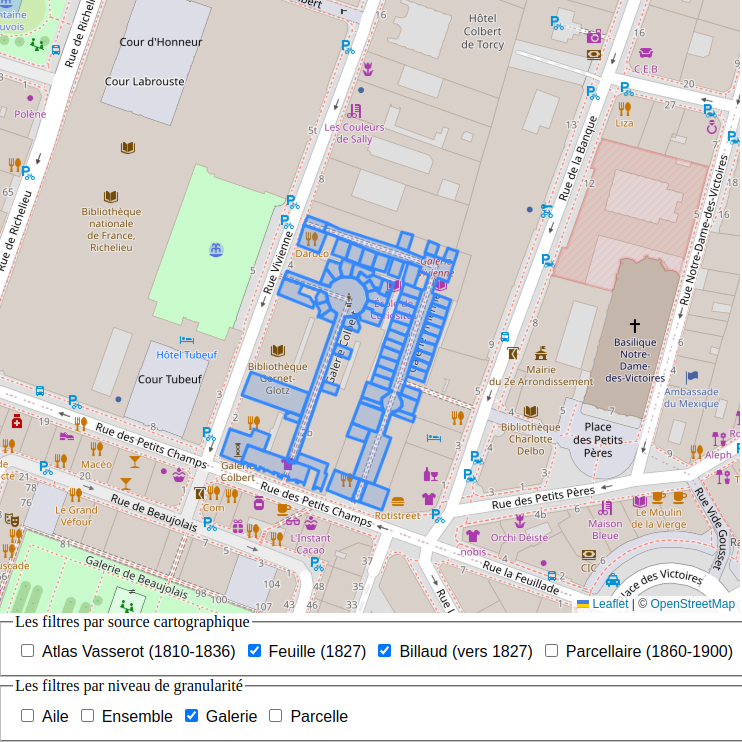
\includegraphics[width=0.7\linewidth]{images/gran-galerie.png}
    \caption{Affichage par galerie}
    \label{fig:gran-galerie}
    \end{subfigure}
    \caption{Exemple d'affichage sans et avec formatage précisé des données de lieux}
\label{fig:granularité}
\end{figure}

Le code est ainsi récupéré par une fonction \texttt{fetch()} qui prend en arguments \texttt{data} et \texttt{category}, représentant respectivement la donnée et la catégorie associée. Ces variables sont ensuite liées à un élément \acrshort{html} \texttt{checkbox}, un ensemble de cases à cocher, dont chaque catégorie possède son identifiant. Une fonction JavaScript est ensuite déclenchée pour afficher les données en fonction de la \texttt{box} cochée.

Cependant, nous avons rapidement constaté que cette approche présente certains inconvénients, comme illustré par la figure \ref{fig:gran-tout}. L'interprétation des données devient complexe. En effet, lorsque tous les paramètres sont sélectionnés, les données s'agrègent, mais les polygones issus des différentes sources cartographiques se superposent, révélant un décalage significatif. Que peut signifier ce phénomène ? Il semble que ces écarts reflètent les divergences entre les sources historiques et les variations dans les niveaux de détail ou de granularité. Il y a donc un polygone par source cartographique et par niveau de granularité, et ces polygones ne correspondent pas toujours parfaitement. Cela est probablement dû à l'utilisation de projections cartographiques différentes lors du géoréférencement des polygones dans le \acrshort{sig}.

\begin{figure}[h!]
    \centering
    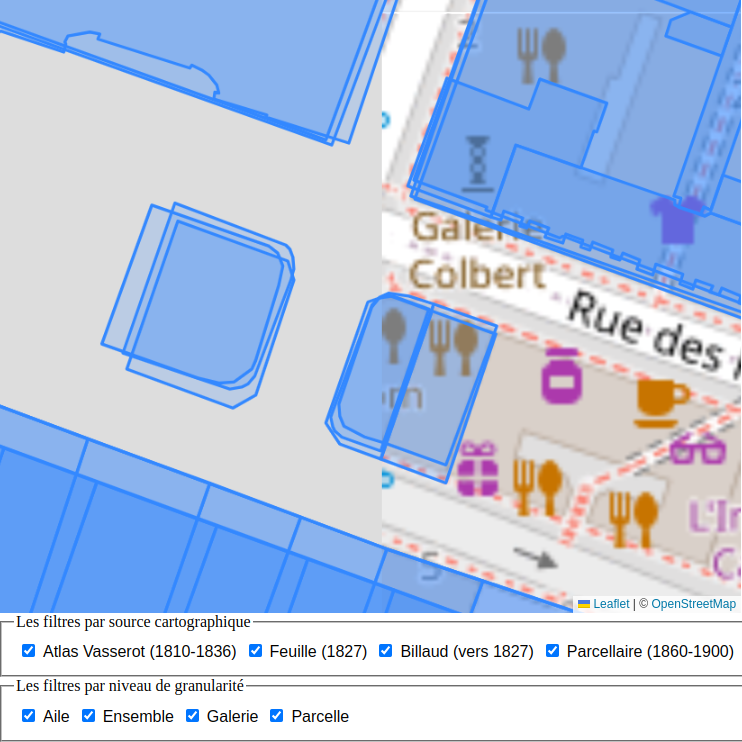
\includegraphics[width=0.4\linewidth]{images/gran-tout.png}
    \caption{Toutes les granularités sélectionnées}
    \label{fig:gran-tout}
\end{figure}

Finalement, requêter à partir de la table \texttt{Place} est la solution la plus adéquate car elle fournit une structure complète, unique et cohérente du lieu comme entité géographique et elle centralise toutes les informations liées. 

\subsubsection{Une figuration de la densité d'information : \textit{heatmap} parcellaire}
Pour se concentrer sur la notion de lieu, nous proposons de représenter la densité d'informations iconographiques liées à chaque lieu. Il s'agit d'une \textit{heatmap} parcellaire ou carte de chaleur, où la \enquote{chaleur} est représentée par la couleur de chaque parcelle ou zone sur la carte, en fonction du nombre de sources iconographiques associées. Cette proposition s'apparente donc à une carte choroplèthe zonale.

\begin{figure}[h!]
    \centering
    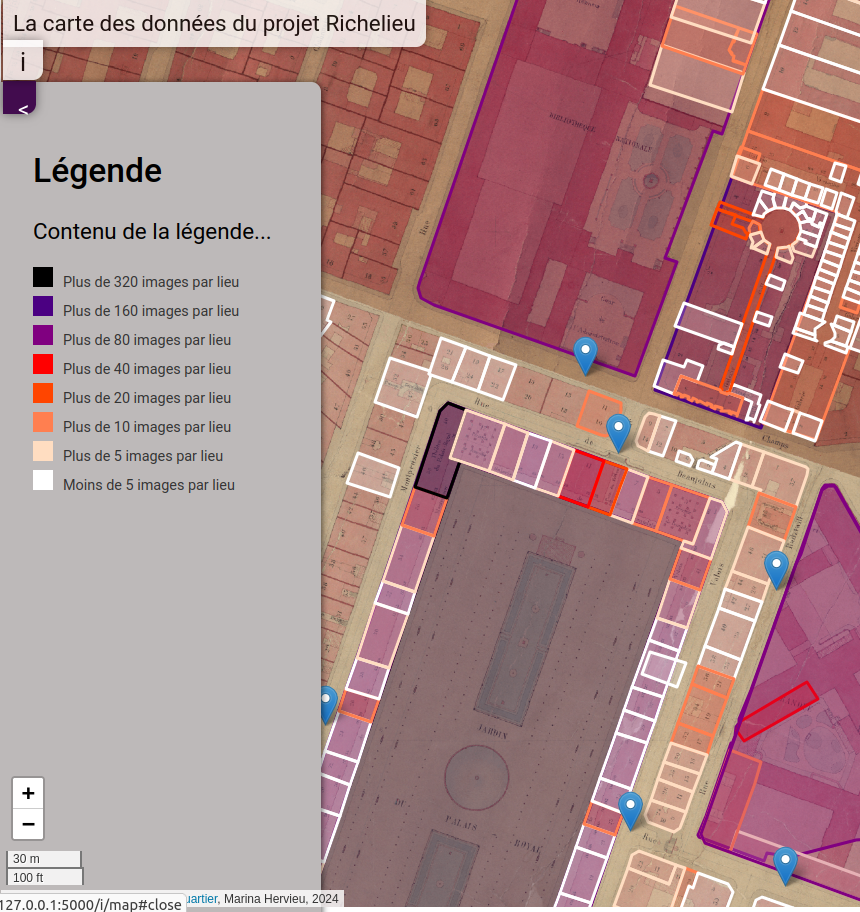
\includegraphics[width=0.75\linewidth]{images/heat-map-density.png}
    \caption{\textit{Heatmap} parcellaire pour la densité d'informations iconographiques, accompagnée de sa légende}
    \label{fig:heat-map}
\end{figure}

Le code en question utilise la fonction \texttt{fetch('/api/places')} présentée dans la section \ref{sous-section:fetch-api-places} pour récupérer les données GeoJSON des lieux à partir de l'\acrshort{api}. Cette requête a la particularité de comptabiliser le nombre d'iconographies par lieu. Une fois ces données obtenues, elles sont stylisées en fonction de la densité d'informations présentes pour chaque lieu. Chaque polygone (représentant une parcelle) est coloré en fonction du nombre d'iconographies associées, grâce à la fonction \texttt{getColorForCount(count)}. Par exemple, une parcelle avec plus de 320 iconographies sera colorée en noir, tandis qu'une autre avec moins de 5 iconographies sera blanche. Comme l'indique le tableau ci-suit(\ref{tab:legende}), beaucoup  de lieux possèdent entre 1 et 5 iconographies, avec une décroissance rapide au~-~delà. Pour définir les seuils de couleurs dans la légende, nous avons utilisé une fonction exponentielle de la forme $5 \times 2^n$. Cette approche permet de visualiser rapidement la concentration des sources iconographiques dans certaines zones : plus la couleur est foncée, plus la densité de sources est élevée.

\begin{table}[!]
    \centering
    \begin{tabular}{|l|c|}
    \toprule
        \textbf{Nombre d'iconographies} & \textbf{Nombre de lieux}\\
    \midrule
         5  & 149 \\
         10 & 60 \\
         20 & 43 \\
         40 & 17 \\
         80 & 13 \\
         160 & 9 \\
         320 & 6 \\
         < 320 & 2 \\
        \bottomrule
    \end{tabular}
    \caption{Calcul du nombre de lieux par nombre d'iconographies}
    \label{tab:legende}
\end{table}
 
La carte permet ainsi de visualiser la répartition inégale des sources cartographiques et iconographiques par lieu - pour des raisons que nous avons déjà expliquées (voir \ref{sous-section:lieu}). En effet, une première analyse de la répartition des sources (figurée dans un camembert ou d'autres graphiques) montre que la majorité des sources est concentrée sur un petit nombre de lieux. Cela correspond également à l'affichage sur la carte, où certaines parcelles apparaissent plus denses en informations, tandis que la majorité des lieux possède beaucoup moins de données. On remarque aisément en noir le \enquote{RM 19}, soit le 19, rue Montpensier (voir le paragraphe correspond \ref{sous-sous-section:rm19}). Cette carte de chaleur met donc en lumière une distribution déséquilibrée des sources, avec une forte concentration d'iconographies et de documents sur quelques lieux emblématiques. 


\subsubsection{Les images liées}
Enfin, il convient de faire apparaître par lieu les iconographies qui y sont liées. Elles sont visualisées sur la carte de façon interactive. 

\begin{figure}[h!]
    \begin{subfigure}{.5\textwidth}
      \centering
    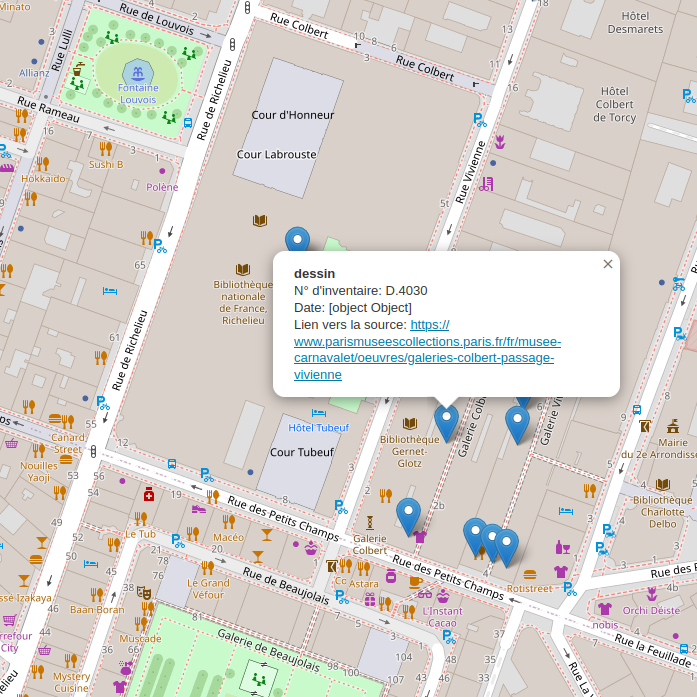
\includegraphics[width=.7\linewidth]{images/pop-up-old.png}
    \caption{Pop-up essai n°1 }
    \label{fig:pop-up-old}
    \end{subfigure}
    \begin{subfigure}{.5\textwidth}
      \centering
    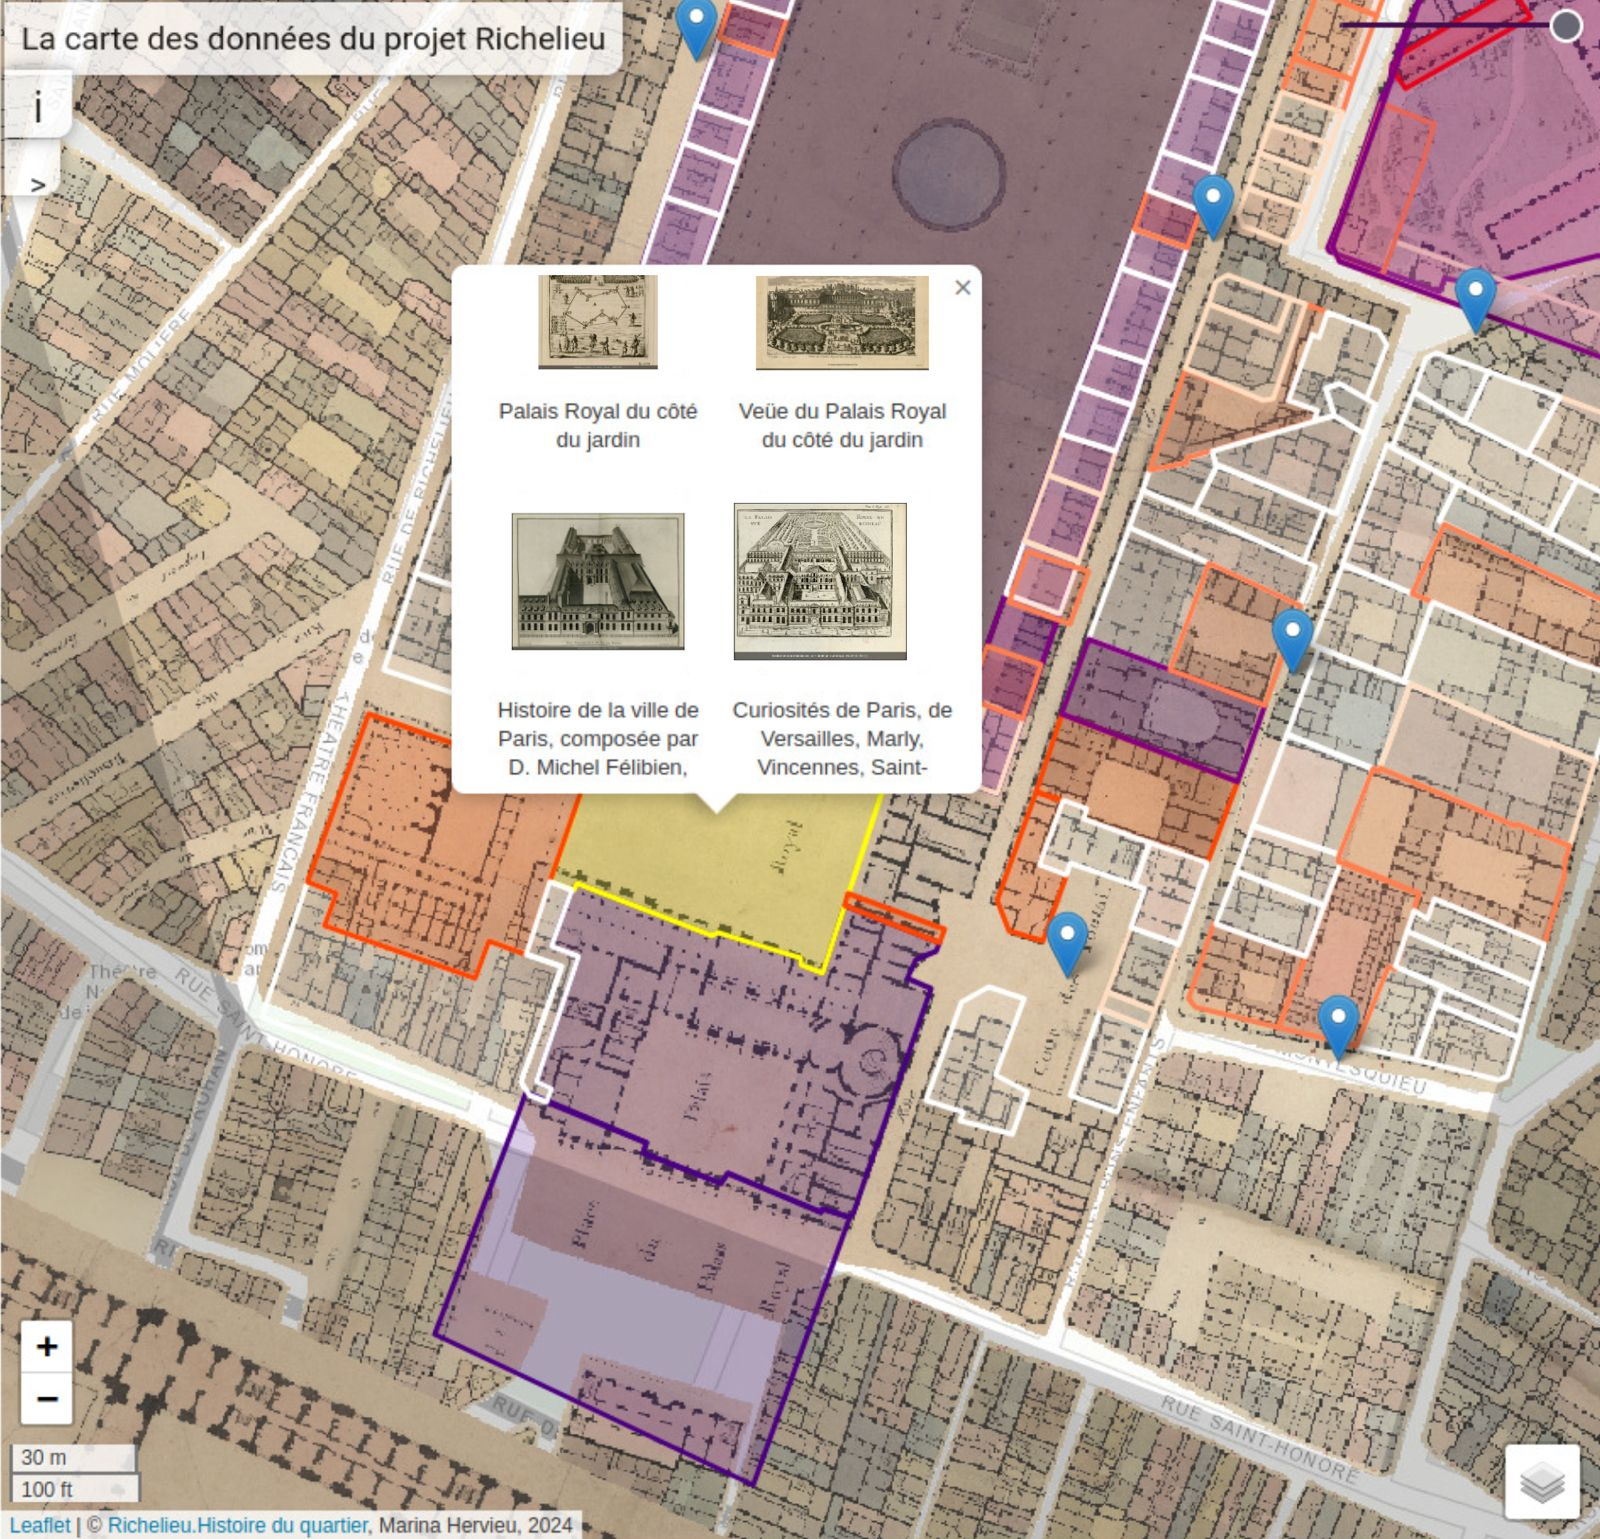
\includegraphics[width=.7\linewidth]{images/pop-up.jpeg}
    \caption{Pop-up essai n°2}
    \label{fig:pop-up}
    \end{subfigure}
    \caption{Exemple d'affichage des iconographies liées aux lieux}
\label{fig:pop-up-all}
\end{figure}

Lorsqu'un utilisateur clique sur un des points dans la figure \ref{fig:pop-up-old} ou sur une des parcelles comme dans la figure \ref{fig:pop-up}, un pop-up s'ouvre pour afficher des informations détaillées (le titre, l'auteur, la date de création, le numéro d'inventaire, etc.) sur le lieu ainsi que les iconographies associées. Le code ci-dessous permet d'afficher une galerie d'images directement dans le pop-up, avec les données récupérées pour chaque lieu. Chaque image dans la galerie est liée à une source iconographique via une \acrshort{url} \acrshort{iiif}. Si l'utilisateur rencontre un problème pour afficher en miniature les images \acrshort{iiif}, il peut cliquer sur l'encart qui devrait accueillir l'image, alors elle s'ouvre dans un nouvel onglet. Cet effet n'est pas un paramètre par défaut de Leaflet et correspond à l'élément \acrshort{html} \texttt{alt} dans le code ci-dessous. Si plusieurs titres sont associés à une image, alors une galerie d'images est générée et elles sont combinées et affichées en deux colonnes, permettant à l'utilisateur d'explorer visuellement les ressources liées à ce lieu sans entraver l'exploration sur le reste de la carte. De plus, le polygone change de couleur quand il a déjà été visité (il devient jaune). Ce mécanisme est illustré dans le figure \ref{fig:pop-up}. Il permet à l'utilisateur de se situer sur la carte. 

\begin{lstlisting}[language=HTML, caption=Création d'un pop-up et d'une galerie d'images]
function showImageGalerie(placeId, layer, iconographies) {
    if (iconographies && iconographies.length > 0) {
        var galerieHtml = '<div class="popup-galerie">';
        iconographies.forEach(function(iconography) {
            var sourceUrl = iconography.source_url || '';  /
            var title = iconography.title ? iconography.title.join(', ') : 'Untitled';  
            galerieHtml += '<div class="popup-galerie-item">';
            galerieHtml += '<img src="' + sourceUrl + '" class="popup-galerie-image" alt="' + title + '"/>';  
            galerieHtml += '<p>' + title + '</p>';  
            galerieHtml += '</div>';
            });
        galerieHtml += '</div>';
        layer.bindPopup(galerieHtml, { maxHeight: 300 }).openPopup();
        } else {
        layer.bindPopup('<p>Il n'y a pas d'images liées à ce lieu.</p>').openPopup();
        }
    }
\end{lstlisting}
Ce code JavaScript définit la fonction \texttt{showImageGalerie}. Un conteneur \acrshort{html} est créée pour contenir la galerie d'images. Ce conteneur est initialisé avec une \texttt{div} de la classe \texttt{popup-galerie}. Puis une boucle \texttt{iconographies.forEach} parcourt chaque iconographie associée au lieu cliqué pour créer un élément \acrshort{html} pour chacune des iconographies. Enfin une variable vient récupérer et stocker l'\acrshort{url} de l'image et la variable \texttt{title} récupère le titre. Puis, un élément \acrshort{html} est généré pour chaque item de la galerie dont l'\texttt{img src} (\acrshort{url} pointant vers la source de l'image) et un texte alternatif, défini par l'attribut \texttt{alt}, s'affiche lorsque l'image ne peut pas être chargée. Puis la galerie d'images est fermée avec la \texttt{</div>}.
Pour afficher la galerie dans un pop-up, un cartel interactif, on utilise une fonctionnalité de Leaflet \texttt{bindPopup} qu'on associe au contenu \acrshort{html} \texttt{galerieHTML} généré juste avant. Un message informationnel est aussi ajouté en cas d'absence d'image liée au lieu. A travers ce code, on propose de créer automatiquement les éléments \acrshort{html} via le JavaScript. 

Finalement, ce système de visualisation dynamique permet une exploration intuitive des lieux en relation avec leurs iconographies historiques, renforçant ainsi l'engagement avec les données géographiques et patrimoniales. 

\subsubsection{Des initiatives à l'état de brouillon}
Les développements mentionnés précédemment ne représentent que quelques exemples parmi d'autres initiatives. Un \textit{slider} temporel a notamment été implémenté pour afficher les parcelles correspondant aux images associées à la date sélectionnée. Toutefois, le résultat final s'est révélé peu satisfaisant , car les données ont effectivement été écrasées (comme anticipé au chapitre \ref{sous-sous-section:chrono}), et le manque de temps a constitué une contrainte pour résoudre ce problème.Ainsi il semble en effet complexe de combiner de manière fluide l'ensemble des axes de recherche – temps, espace et iconographie – sur une seule carte. Une approche alternative pourrait consister à proposer des mini-cartes encapsulées dans la carte principale, offrant ainsi une visualisation plus spécifique et ciblée\footnote{La carte Artl@s est disponible \href{https://paris-art-market.huma-num.fr/}{ici} opte pour cette solution par exemple.}. Il y aurait une carte principale qui propose en option, une carte visualisant la granularité des données; puis une carte visualisant la densité des données. Par ailleurs, le développement de filtres thématiques, ainsi que la fonctionnalité de sélection et de sauvegarde de zones, n'a pas pu être mené à terme. Toutefois, selon le \acrshort{mvp}, les fonctionnalités en orange ont toutes été développées. 

\subsubsection{Conclusion du chapitre}
Pour conclure, nous avons vu que la réalisation technique de la carte s'inscrit dans un processus de développement  \textit{full-stack} en plusieurs étapes, débutant par la définition des fonctionnalités structurelles via la bibliothèque Leaflet, comme le fond de carte, le cartouche et les éléments interactifs. La connexion à la base de données a ensuite été établie grâce à une \acrshort{api} REST, permettant de récupérer et d'afficher dynamiquement les données sur la carte, offrant une exploration interactive des lieux et des iconographies du projet Richelieu. L'intégration des fonds de carte et des couches superposées a permis une gestion en temps réel de la visibilité des informations, tandis que la connexion à la base de données a enrichi la carte avec des données dynamiques. Le rôle central de l'\acrshort{api} REST a facilité l'échange de ces données, démontrant ainsi la flexibilité et l'efficacité de cette architecture pour offrir des visualisations variées, tout en maintenant la connexion avec les sources historiques. Ce chapitre souligne l'importance de la cartographie Web interactive pour rendre les données historiques plus accessibles, tout en les ancrant dans la réalité du projet.

\subsubsection{Conclusion de la deuxième partie}
Dans cette deuxième partie, les différentes étapes de la conception et du développement de la carte Web en tant qu'outil d'exploration des données ont été exposées. Grâce à une approche méthodique, nous avons défini les objectifs de visualisation des données en lien avec le projet Richelieu, tout en prenant en compte les contraintes techniques et les attentes fonctionnelles. La visualisation des données du projet Richelieu s'effectue à travers une carte choroplèthe, offrant diverses possibilités pour varier l'affichage selon la densité ou la granularité. Cependant, elle ne peut intégrer la dimension de réseau, bien que cela ait été souhaité au départ du projet. De plus, la représentation précise de la dimension temporelle reste complexe et limitée en moyen tant humain que temporel.

La carte présente néanmoins un avantage majeur, en ligne avec la vision de Malraux et de son musée imaginaire\footcite{MALRAUXMusee1996} : dans un espace restreint, à l'échelle d'un quartier, elle réunit un nombre considérable de sources iconographiques et cartographiques provenant de diverses institutions, y compris étrangères. Toutefois, la carte ne peut offrir une visualisation exhaustive : elle n'affiche pas toutes les informations associées à une image. Or, l'histoire de l'art étant une discipline rigoureuse, il est essentiel de mentionner les sources, les techniques, la datation et d'autres informations qui ne peuvent être pleinement lues sur la carte à défaut de la rendre illisible. Cependant, la cartographie sur le Web permet d'accéder, d'un simple clic, à l'ensemble de ces données complémentaires grâce à un renvoi vers la page principale de l'image qui détaille ces informations sur le site du projet Richelieu.

Quant à savoir si la carte est avant tout une \textit{démonstration} ou un objet de \textit{recherche}, ou peut-être les deux, comme le suggère Grandjean, il revient aux utilisateurs, d'une part, et, aux chercheurs d'autre part,  d'explorer cet outil pour déterminer s'il offre de nouvelles perspectives de recherche sur le quartier Richelieu.